\documentclass[a4paper,10pt]{article}

\usepackage{inputenc}
\usepackage[francais]{babel}
\usepackage[T1]{fontenc}

\makeatletter
\def\sanstitre{\def\section{\@ifstar\@gobble\@gobble}}
\makeatother

\usepackage{eurosym}

%% Sans-serif Arial-like fonts
%\renewcommand{\rmdefault}{phv} 
%\renewcommand{\sfdefault}{phv} 
\usepackage{tabularx}
\usepackage{graphicx}
\usepackage{eurosym}
\usepackage{xspace}
\newcommand{\projectname}[0]{DADA\xspace} 
\usepackage[colorlinks,linkcolor=blue,citecolor=blue,urlcolor=blue]{hyperref}
\setlength{\footskip}{2cm}
\setlength{\headheight}{2cm}
\usepackage[lmargin=2.5cm,rmargin=2.5cm,tmargin=3.5cm,bmargin=1.5cm,includefoot]{geometry}  
\usepackage{lastpage}%% to get the total number of pages

\usepackage{pdflscape}


\usepackage{fancyhdr}
\pagestyle{fancy}
\fancyhfoffset[re]{4cm}

\lhead{}
\rhead{Appel \`a Projet G\'en\'erique - Projet \projectname  - \'Edition 2015  - Document scientifique}
 

\lfoot{ANR 2015 - DADA - Doc Scientifique}
\cfoot{}
\rfoot{\thepage/\pageref{LastPage}} 


\newcommand{\mytitle}{Latex Skeleton for ANR}

\title{\mytitle}

\title{Directing Autonomous Digital Actors}

\newcommand{\content}[1]{\emph{#1}\\} 

\bibliographystyle{abbrv}

% http://nw360.blogspot.com/2007/12/rename-bibliography-title-in-latex.html
\renewcommand\refname{\vspace{-1cm}}



\usepackage{xcomment}
%%\newenvironment{xcomment}{\em}{}

\begin{document}

\maketitle

\begin{xcomment} 
Warning: the comments are turned on. All directives and guidelines appear.\\
To turn them off, comment the line   \verb|\newenvironment{xcomment}{\em}{}|\\
and uncomment the line  \verb|\usepackage{xcomment}|
\end{xcomment} 



%% PAGE 2 with table
%\begin{landscape}
%\thispagestyle{empty}
 
%% PAGE 3 Table des mati\`eres (obligatoire)
\setcounter{tocdepth}{2}
\tableofcontents
\newpage


\section{R\'esume de la proposition de projet / Executive summary}

\begin{xcomment}  
Recopier le r\'esum\'e utilis\'e dans le document administratif et financier.
\end{xcomment}

Character animation has been tackled through various approaches in the past. To name a few, chosen among those that are directly related to DADA, we can cite: embodied conversational agents (ECA); statistical models learned from motion capture examples; physically-based animation; and speech-driven animation. Very few attempts have tried to merge these various approaches into a single model offering on one hand expressive animation and on the other hand high control over the animation. In order to make progress in the field, we propose to shift the focus from autonomous characters to autonomous actors. Autonomous characters make decisions based on AI models of their personality and goals. In contrast, autonomous actors follow a precise script, written by the director, while adapting their behaviors autonomously to the virtual environment they are placed in that includes objects and other actors. 

The goal of the DADA project is to design, implement and evaluate novel interfaces for directing expressive, autonomous virtual actors, borrowing from established theatre practices. We will combine fundamental research in 3D animation, machine learning and intelligent agent programming to leverage motion capture data sets of professional actors into a virtual theatre company of synthetic actors with acting skills, i.e. ability to respond to a director�s instructions and to perform together on a virtual stage. Virtual theatre will be used as a test application for obvious extensions to other digital storytelling applications.

To reach this ambitious goal, DADA will learn parameterized models of actor�s movements and gestures from existing annotated motion capture databases of actor performances; and create intuitive authoring tools for creating a script of actions and cues in a machine-readable format suitable to real-time control of the virtual actors. More precisely, the academic partners of the project will engage fundamental research along two main directions:

\begin{enumerate} 
\item Animating autonomous actors procedurally. A key idea in DADA is to separate the animation model into a proxemic component regulating how actors interact with each other and the audience, and a kinesic component regulating how actors use their body language to communicate moods and expressions (Tannenbaum 2014). The proxemic component of animation will drive the positions and orientations of actors on the stage as well as their gaze directions. This component will be driven by a model encompassing the social relations between and the emotional attitudes of the autonomous actors. The kinesic component of animation will drive all other degrees of freedom of the virtual actors. This component will be driven by parametric statistical models trained from an existing motion capture data-set. The separation between the two components is expected to yield important benefits in terms of expressivity and composability.

\item Synchronizing virtual actors to a single story-line using a story-driven architecture of actors following a scripted sequence of instructions. In contrast to previous works, which used programming languages, we will investigate multimodal interfaces offering directorial control in a high-level, pseudo-natural language familiar to the director. The language will be compiled internally to a finite-state machine representation controlling the real-time execution of the autonomous actors. 
\end{enumerate}


All developments will be validated by experiments with the theatre department of Paris 8. Starting from a selection of play scripts in various genres and with increasing complexity, theatre experts will use the DADA tools to create virtual theatre performances in the Unity game engine, including stage movements and actions (entering, exiting, sitting down, standing up, taking and putting objects on the stage); body language expression of the personalities, moods and emotions of the characters; and believable gaze, proxemics and action/reaction behaviors between actors.
\section{Introduction et positionnement / Introduction and positioning}

\subsection{Contexte et enjeux \'economiques et soci\'etaux / Context, social and economic issues}
\begin{xcomment}  
D\'ecrire le contexte \'economique, social, r\'eglementaire' dans lequel se situe le projet en pr\'esentant une analyse des enjeux sociaux, \'economiques, environnementaux, industriels' Donner si possible des arguments chiffr\'es, par exemple, pertinence et port\'ee du projet par rapport à la demande \'economique (analyse du march\'e, analyse des tendances), analyse de la concurrence, indicateurs de r\'eduction de coûts, perspectives de march\'es (champs d'application, '). Indicateurs des gains environnementaux, cycle de vie'
\end{xcomment}

Creating believable, human-like performances by virtual actors is an important problem in many digital storytelling applications, e.g. creating non-player characters (NPC) for video games, creating expressive avatars in next-generation virtual worlds, populating movies and architectural simulations with background characters and crowds, creating believable virtual tutors and coaches in educational serious games, and creating believable characters for interactive fiction and interactive drama. A desirable feature for such applications is the ability to create virtual actor performances which are both expressive and controllable. Motion capture actors are expressive, but once recorded, their performances cannot easily be controlled, edited or modified. As a result, game companies ought to get engaged in extensive motion capture sessions of all actions and moods of all characters in every new game they create. On the other end of the spectrum, procedural 3D animation can be controlled in every detail using sophisticated programming techniques, but they fall short of providing the level of expression required for conveying the subtle inflexions of human-like performances.

Character animation has been tackled through various approaches in the past. To name a few, chosen among those that are directly related to DADA, we can cite: embodied conversational agents (ECA), ie autonomous virtual characters \cite{Cassell2000}; statistical models learned from motion capture examples \cite{Lee2002}; physically-based animation \cite{Liu2006}; and speech-driven animation \cite{Ding2013}. Very few attempts have tried to merge these various approaches into a single model offering on one hand expressive animation and on the other hand high control over the animation. In order to make progress in the field, we propose to shift the focus from autonomous characters to autonomous actors. Autonomous characters (such as The Sims) make decisions based on AI models of their personality and goals. In contrast, autonomous actors follow a precise script, written by the director. Their autonomy is therefore limited to perform-ing a precise sequence of actions as a result of various cues  written in the script. Creating such performances procedurally using autonomous actors is a valuable goal because it would make it possible for each performance to be unique, which is widely regarded as an important quality to ensure liveliness and immersion, while maintaining a high level of directorial control. Merging both approaches would allow creating autonomous actors able to follow a script (specified in high-level command-like language) that give the main directions the actors ought to follow while adapting their behaviors autonomously to the virtual environment they are placed in that   includes objects and other actors.



\subsection{Positionnement du projet / Position of the project}
\begin{xcomment}  
Pr\'eciser :
positionnement du projet par rapport au contexte d\'evelopp\'e pr\'ec\'edemment : vis- à-vis des projets et recherches concurrents, compl\'ementaires ou ant\'erieurs, des brevets et standards'
indiquer si le projet s'inscrit dans la continuit\'e de projet(s) ant\'erieurs d\'ejà financ\'es par l'ANR. Dans ce cas, pr\'esenter bri\`evement les r\'esultats acquis,
positionnement du projet par rapport aux axes th\'ematiques de l'appel à projets,
positionnement du projet aux niveaux europ\'een et international.
\end{xcomment}


Animating virtual agents with expressivity is a grand challenge for the entertainment industries (video games, movie industry) that rely mainly on motion capture data which allows them to produce rich and subtle motion but with a high cost in time and finance. On the other hand, technology for interactive agents uses mainly procedural approach. While such approach allows modulating in real-time agents' motion and its quality, the results are still far from being natural and realistic. Lately statistical approaches have been developed. They are promising as they produce animations captur-ing naturalness and richness of human motion. However the control of such animation technique is still an issue and its extension to a large range of motion activities is also an important challenge.

DADA aims to bridge the gap between those previous techniques by proposing a general framework for combining them into a unified interface. A desirable outcome of the project will be a completely novel interaction model for rehearsing with virtual actors and incrementally building complex multi-actor performances with multiple layers of 3D animation. Thus DADA fits the component Information and Communication Society; it is also in line with at least two axes of the ANR call.

\begin{itemize}
\item[First axis:] Le num\'erique au service des arts, du patrimoine, des industries culturelles et \'editoriales (3.7.1.3). There are several potential applications of DADA on top of the proposed virtual theater. The creation of expressive virtual characters can be used in video games, especially for NPC (non-player characters), and in serious games. Indeed being able to simulate the motion of a virtual actor with different expressivities and for different morphologies while maintaining a high level of naturalness and lifelikeness will be a big benefit in time and money.

\item[Second axis: ] Interactions des mondes physiques, de l'humain et du monde num\'erique (3.7.2.4). The outcome of DADA
will benefit the creation of virtual agents, either autonomous or controlled by humans. These agents ought to display a
large variety of communicative and emotional expressions toward human interactants as well as to perform many actions with objects in their virtual environment. Enhancing, in quantity and expressivity, the behaviors of virtual agents is one of the challenges of DADA that falls under the axis.
\end{itemize}

\paragraph{Related projects:} There exist several large European projects that are related to DADA research themes. However, to our knowledge, none covers our research question of building expressive animation with different levels of control. We can name the NoE IRIS on story-telling, the IP Companions on dialog virtual agents, the IP REVERIE on modeling virtual characters in highly immersive virtual environment, and the STREP Ilhaire aims to simulate laughing agent using data-driven and motion graph approaches. On the National side, we can name the Feder project Anipev in which the database Emilya has been captured.

Several recent projects have been devoted to the interface between computers and theatre, e.g. ANR VIRAGE (a generic architecture for controlling lighting and music during theatre production), ANR OSSIA (authoring tools for writing interactive, multimedia scenarios) and ANR INEDIT (INteractivit\'e dans l'Ecriture De l'Interaction et du Temps). ANR Spectacle-en-ligne(s) was a SHS CORPUS project dedicated to capturing, indexing and annotating 200 hours of theatre rehearsals recorded in high-definition video. Those projects focus on the interaction of computer systems with real actors. In contrast, DADA will focus on the core issue of directing virtual actors.

Despite considerable academic research, few procedural animation systems have become commercially available in recent years. Euphoria by Natural Motion is a real-time procedural animation engine, which has been used in Grand Theft Auto 4 and other games. However, actions and expressions are difficult to control. Xtranormal Technologies was an online service for quickly creating 3-D animations from dialogues decorated with stage directions, using a proprietary procedural animation engine limited to non-expressive behaviors.  Actor Machines is a company created by Ken Perlin to commercialize packages of trained virtual actors  with a large range of actions and expressions, which has not delivered any product yet.



\subsection{Etat de l'art / State of the art}
\begin{xcomment}  
Pr\'esenter un \'etat de l'art national et international, en dressant l'\'etat des connaissances sur le sujet. 
Faire apparaître d'\'eventuelles contributions des membres de la proposition de projet à cet \'etat de l'art.
Faire apparaître d'\'eventuels r\'esultats pr\'eliminaires. 
Inclure les r\'ef\'erences bibliographiques n\'ecessaires au � 7.
\end{xcomment}

A large body of theoretical research work relates to acting and directing in the theatre, especially from a cognitive science
perspective \cite{Kemp2010}. Its applicability to virtual actors is limited because of the huge gap between virtual and human acting skills.
An extensive survey of acting techniques used in 3D animation and virtual worlds can be found in the excellent collection edited 
by Tanenbaum, et al. \cite{Tanenbaum2014}. The priomises and limitations of virtual actors  in contemporary 
theatre has been surveyed by Dixon \cite{Dixon2007}, Salter \cite{Salter2010} and Bourassa and Poissant \cite{Bourassa2013}.


\subsubsection{Single-character animation}

Animation of an avatar is usually tackled by working separately on the full body animation model on the one hand and on the face (and gesture) animation model on the other hand (since the latter animation strongly depends on the dialogue the avatar is engaged in), where the animation produced by the two models are merged to produce a final complete animation \cite{DBLP:journals/tvcg/ShoulsonMKB14}. 

Full body kinematic animation (or control) consists in animating the full body of an avatar while he is performing actions such as walking, dancing, sitting etc. Although there has been lots of work on this subject it is still a challenging problem due to the high dimensionality of the character's configuration. Data-driven approaches are very popular here and make of use motion-capture data to learn 
animation models which, once learned, may be used to animate a virtual character to perform a given task. Many animation techniques based on concatenation of motion capture data and clips selection~\cite{Lee:2002:ICA,Kovar:2002:MG,Heck:2007:PMG} have been proposed. These methods focus on how to improve the clips searching performance or the transition quality between successive clips. These methods have been applied very successfully to locomotion synthesis. Feng et al.~\cite{Feng:2012:EMS} have extended motion example method for gesture synthesis.
Since they use directly motion capture, their synthesized result is quite natural, but do suffer from some limitations: new data needs to be recorded for any new required animation.

 
Many systems have been proposed for producing animation models and controlers, they usually are based on statistical models such as Hidden Markov Models (HMMs) \cite{DBLP:journals/tog/LevineTK09} and Conditional Random Fields (CRFs) \cite{DBLP:journals/tog/LevineKTK10, DBLP:conf/atal/ChiuM14}. Most accurate methods exploit a large dataset of motions where one can synthesize a complete motion sequence corresponding to a particular task by using warping or blending strategies of motions in the training set \cite{DBLP:conf/siggraph/WitkinP95}. Locomotion controllers have been proposed that concatenate motion clips from a motion capture dataset to produce an animation that is smooth \cite{DBLP:journals/tog/TreuilleLP07, DBLP:journals/tog/McCannP07}. High-quality kinematic controllers have been built from this idea by using a {\it motion graph}, which is a graph structure that describe how clips from a dataset can be reordered into new motions \cite{DBLP:journals/tog/LeeCRHP02}. 


Style Machines~\cite{Brand:2000:SM} achieve the stylistic motion synthesis by learning motion patterns from a highly varied set of motions, as a distinct choreography can perform motions with a distinctive style. Stylistic Hidden Markov models (SHMM) are proposed to train different stylized behaviors. A new style motion can also be obtained from the interpolation of SHMM sub-spaces. This approach treats animations as a pure data modeling task. Later, such types of work have been extended~\cite{Wang:2003:LKH}~\cite{Pan:2009:UHM}, but, so far, the focus of these  synthesis works is more on cyclic motion; cyclic motions are somehow easier to treat for clustering, blending or filling missing data. 

While locomotion controllers are driven by direct high-level commands (such as desired movement direction), no such clear control signal is available for body language. To animate the face, and accompanying arm gestures, many works have focused on developing specific animation models based on a dialogue related input, either speech, text or prosody features \cite{DBLP:journals/tog/LevineTK09, DBLP:journals/tog/LevineKTK10, DBLP:conf/atal/ChiuM14, ding2014upper}.  Finally, recent work has demonstrated such models for the case of locomotion believable controllers, gesture controllers \cite{DBLP:journals/tog/LevineKTK10} and face controllers \cite{DBLP:conf/icassp/DingRAP13}. 

% We will aim to generalize this previous work
% to more general action controllers, including such actions as: sitting, standing, walking, grasping, taking and putting
% objects, in a variety of expressions and moods.
Yet all these statistical approaches require large annotated datasets to work well. Thereby these approaches do not easily work with small training sets which is a key issue, as stressed for instance in \cite{DBLP:journals/tog/LevineWHPK12}, since first it requires considerable effort and time to build large datasets, and second because many applications demand unique motion styles and require their own datasets. This has led a number of researchers to put the effort on designing models that may be easily learned from a few samples. One main approach for doing so lies in the use (or learning) of a continuous state space to represent the data, making learning in this low dimensional space much easier  \cite{DBLP:journals/tog/LevineWHPK12, DBLP:conf/atal/ChiuM14}. A relevant technology for this are Gaussian Process which have been extended for dealing wiuth dynamic data in \cite{DBLP:journals/pami/WangFH08}.

These latter models are not far from recurrent neural networks, and to Long Short Term Memory neural networks in particular \cite{DBLP:conf/nips/HochreiterS96, DBLP:journals/corr/GreffSKSS15}, that have been shown recently to work well for complex signals such as speech and handwriting, for recognition tasks \cite{DBLP:conf/nips/GravesS08} as well as for synthesis tasks \cite{DBLP:journals/corr/Graves13}. These models are part of a current trend in machine  learning called representation learning (see the recently born conference ICLR at http://www.iclr.cc/) which aims at discovering relevant and usually low dimensional representation of the data under investigation (the pionner work of this domaine is the one by G. Hinton in Science \cite{DBLP:journals/cogsci/HintonOWT06}.

\subsubsection{Multiple-character animation}

\paragraph{ECAs gathering in groups}: Prada and Paiva \cite{PradaPaiva05} modeled groups of autonomous synthetic virtual agents that collaborated with the user in the resolution of collaborative tasks within a 3D virtual environment. Rehm and Endrass \cite{RehmEndrass09}  implemented a toolbox for modeling the behavior of multi-agent systems. In \cite{RavenetCOP14}, Ravenet and colleagues combined a number of reactive social behaviors, including those reflecting personal space \cite{Hall69} and the F-formation system \cite{Kendon90}, in a general steering framework inspired by \cite{Reynolds99}. This complete management of position and orientation is the foundation of the Anonymous Engine used in the work presented here. All these models did not take into account the expression of attitudes while exhibiting the behaviors of the agents.

Forward Kinematics (FK) and Inverse Kinematics (IK) have been used to generate animation sequences procedurally~\cite{Boulic:2006:EOA,Unzueta:2008:FPA}.
Different constraints and unconstrained numerical equation solvers are used to model the motion postures and their transitions~\cite{Zhao:1994:IKP}. The target based reaching models, such as Jacobian methods~\cite{Yuan:2001:LSI}~\cite{Buss:2004:SDL}, are proposed to use linear approximation to bring the end-effector close to the target; it can be used to build a posture configuration for virtual characters. These methods are flexible and widely used for real time lost cost procedural generation and motion editing, but the resulting motions may not be as realistic as human motion. They can show quite some stiffness. 

There exist several systems embedded in large platform that combine different animation synthesis solutions. The Smartbody system~\cite{Shapiro:BCA}~\cite{Thiebaux:2008:SBR} includes a schedule controller and a realization controller. Smartbody includes different motion synthesis methods such as motion capture data and dynamic system. ETENDRE: DONNER PLUS D INFORMATION. IL FAUT AUSSI EXPLIQUER EN QUOI NOTRE SYSTEME DIFFERE DU LEUR. The behavior engine developed by Marsella et al.~\cite{Marsella:2013:VCP} makes use of Smartbody. This engine embeds a rule-based system that can determine facial expressions and gestures by extracting semantic, pragmatic and rhetorical content from an input utterance. Some behaviors (eg head motion) are also obtained through data-driven model. Luo et al.~\cite{Luo:2009:AGA} proposed a procedural arm gesture model. They improve the quality of the procedural animation by introducing motion capture data for full body animation. ADAPT~\cite{Shoulson:2013:AAD} is also a flexible platform for virtual human characters. This system has been designed as a gaming system for physical reactions.  They use a behavior tree to model human-like behaviors for multi-characters and a Level of Detail character shadows solution is proposed to generate body parts sequentially. Blending technique is applied to compute the movements of different body parts from different Choreographers. While some motion artifacts may appear when doing blending or character motion transition, this animation platform combines various animation techniques. However it has not been focused on communicative and emotional behaviors that are defined by specific temporal patterns.


Existing animation techniques, procedural and data-driven, have pros and cons. With the procedural animation, gestures are described using the symbolic language BML \cite{Kopp2006}. New behaviors can be created very rapidly; but, most of the time, the obtained animation lacks naturalness and fluidity. On the other hand animation from motion-capture data reproduces all human motion subtleties and dynamics; however creating new gesture is more cumbersome as it requires new recording of data and new training. Our aim in DADA will be to develop an embodied conversational agent system that embeds both animation approaches. Communicative behaviors are computed procedurally while socio-emotional behaviors such as emotions are driven from machine-learning techniques (Task 1.2). Both computations involve the same body parts. While the two animation streams are computed separately they need to be merged to produce the final animation output (Task 2.3).  

\subsubsection{Authoring tools and metaphors} There has been previous work on story-driven architectures and directing tools specifically dedicated
for virtual theatre. The desktop theatre by Strassmann \cite{Strassmann1992},  the Improv  system by Perlin and Goldberg \cite{Perlin1996} and the story-driven architecture by Pinhanez \cite{Pinhanez2000} are seminal works in building virtual actors that can be scripted to perform on a virtual stage.  Other early work in Europe includes the Pinnochio \cite{Maiocchi90} and GEIST \cite{Spierling02} projects, which targetted players of interactive games by letting them "play director". The acting capabilities of those early systems are limited and the amount of programming 
needed to produce even the simplest scene is substantial.

Xtranormal Technologies Text-To-Movie was an online application for quickly creating 3D animation by writing dialogues with emoticons, which were automatically
translated into animation using a combination of procedural and data-driven animation. The DRAMA project at the University of Toulouse has also investigated this paradigm.
While automatic text-to-scene animation is a valid research area, it has the disadvantage that it is taking control away from the director. In DADA, we take
a different route, which is offer maximum control to the director over the virtual actors.

MIRAGE \cite{El-Nasr04} is an interactive story generation engine featuring 3D animation of two virtual actors playing the roles of Electra and Archemedis in a tragic style. Actions 
are represented by a verb, and adverb and an actor; and are either controled by the player or generated by the system. Actor's behaviours are organized into dramatic beats with multiple
actions and reactions based on communicative goals. While the focus of MIRAGE is different from DADA, it offers the important insight that actions performed by the virtual actors must be appraised from the point of view of the user (director, audience or player).  This will be used  as a general guideline in DADA as well.  

%The body action and posture coding system (BAP)  \cite{Dael12a} is an extensive description language for body movement on the anatomical level (body parts), the form level (directions and orientations of movements) and the function level (communicative and goal-driven actions). Their work is important for DADA because it offers a catalogue of  expressive gestures used by professional actors in depicting various emotions \cite{Dael12b}. The language makes it possible to precisely annotate body actions in video using the ANVIL annotation tool \cite{Kipp01,KIPP12}.

The Q language \cite{Ishida2002} is an authoring language for writing scenarios involving multiple autonomous agents. While not targeting theatre
as an application, the language borrows heavily from theatre practices and is based on defining  cues that synchronize  the actions and reactions 
of the agents. Q is a dialect of the scheme language and assumes that the scenario writer is familiar with programming. The directing language
for DADA will also be based on cues and actions, but will be extended to include direct user manipulation using a graphical user interface, rather
than a programming interface. Furthermore, animation generated with the Q language was fairly primitive and we plan to offer a more expressive
and extensive description of the actor's full body animation. 

The movie script markup language (MSML) \cite{VanRijsselbergen2009} has been proposed to encode the stucture of movie  and play scripts into scenes, actions and dialogues. One interesting feature of the language is that it includes an animation layer, making it possible to compute a realization of the play script in 2D animation. The synchronization of the various actors and actions
in the play script is performed by generating an Object Composition Petri Net (OCPN) \cite{Little06} for the entire scene. This feature has not been demonstrated with 3D animation, and it will be one of the objective of the DADA project to implement, test and validate the MSML animation layer with multiple autonomous 3D actors in a real-time game engine. 

Petri nets have also been proposed as a high-level specification for virtual actor behaviours \cite{Magalhaes98,Blackwell01},
including the  important case of turn-taking in dialogue and imitation games \cite{Chao11a,Chao11b}. They are also the basis for the interactive 
musical score system developed by the INEDIT project \cite{Allombert08,Marczak11}, which is being extended to multimedia events \cite{Toro12}. 
Petri nets are likely  candidates to become  an internal, intermediate representation  of the performance score in DADA,  between the high level 
commands of the director and the low-level executable finite-state machine of the game engine.   In previous work,  the composer or director 
manipulates the Petri nets directly. In DADA, we will instead offer direct manipulation of cue sheet  and prompt books, which offer  more natural 
interaction for theatre directors than Petri net places and transitions. 

\subsubsection{Robotic actors}

Our project is also related to the emerging field of  robotic actors performing theatre on a live stage  \cite{Lin2013}. An international workshop was dedicated to
robotics and theatre at ICRA 2012 \footnote{Robotics and Performing Arts: Reciprocal Influences, http://www.robotics-and-performing-arts.sssup.it/}. Our 
research on directing autonomous digital actors will likely be applicable to the case of robotic actors as well. 

\subsubsection{Prior art at LITC}

Our developments will be based on the GRETA platform and use the EMILYA database. The Greta platform simulates virtual agents able to communicate verbally and nonverbally with human users and/or other virtual agents. Given a set of intentions and emotions to be communicated, the platform instantiates them into sequences of synchronized nonverbal behaviours. It can be used to compute these multimodal behaviours when the virtual agent acts as a speaker or as a listener.

The Greta system allows a virtual or physical (e.g. robotic) embodied conversational agent to communicate with a human user \cite{Ochs2013emoti,Niewiadomski2011}. It is a SAIBA compliant architecture (SAIBA is a common framework for the autonomous generation of multimodal communicative behavior in Embodied conversational agents \cite{Kopp2006}). The main three components are: (1) an \textit{Intent Planner} that produces the communicative intentions and handles the emotional state of the agent; (2) a \textit{Behavior Planner} that transforms the communicative intents received in input into multimodal signals and (3) a \textit{Behavior Realizer} that produces the movements and rotations for the joints of the ECA.

A \textit{Behavior Lexicon}  contains pairs of mappings from communicative intentions to multimodal signals. The Behavior Realizer instantiates the multimodal behaviors, it handles the synchronization with speech and generates the animations for the ECA. 

The information exchanged by these components is encoded in specific representation languages defined by SAIBA. The representation of communicative intents is done with the Function Markup Language (FML) \cite{FML2008IVA}. FML describes communicative and expressive functions without any reference to physical behavior, representing in essence what the agent's mind decides. It is meant to provide a semantic description that accounts for the aspects that are relevant and influential in the planning of verbal and nonverbal behavior. Greta uses an FML specification named \textit{FML-APML} and based on the Affective Presentation Markup Language (APML) introduced by \cite{APMLDeCarolis2004}. FML-APML tags encode the communicative intentions following the taxonomy defined by \cite{Poggi2007}, where a communicative function corresponds to a pair (\textit{meaning},\textit{signal}). The meaning element is the communicative intent that the ECA aims to accomplish, whereas the signal element indicates the multimodal 
behavior exhibited in order to achieve the desired communicative intent. The multimodal behaviors to express a given communicative function to achieve (e.g. facial expressions, gestures and postures) are described by the Behavior Markup Language (BML) \cite{Kopp2006}.

%The information exchanged by these components is encoded in specific representation languages defined by SAIBA. The representation of communicative intents is done with the Function Markup Language (FML) \cite{FML2008IVA}. FML describes communicative and expressive functions without any reference to physical behavior, representing in essence what the agent's mind decides. It is meant to provide a semantic description that accounts for the aspects that are relevant and influential in the planning of verbal and nonverbal behavior. Greta uses an FML specification named \textit{FML-APML} and based on the Affective Presentation Markup Language (APML) introduced by \cite{APMLDeCarolis2004}. FML-APML tags encode the communicative intentions following the taxonomy defined by \cite{Poggi2007}, where a communicative function corresponds to a pair (\textit{meaning},\textit{signal}). The meaning element is the communicative intent that the ECA aims to accomplish, whereas the signal element indicates the multimodal behavior exhibited in order to achieve the desired communicative intent. The multimodal behaviors to express a given communicative function to achieve (e.g. facial expressions, gestures and postures) are described by the Behavior Markup Language (BML) \cite{Kopp2006}.

Lately we have been developing data-driven approach to capture the link between acoustic features (speech \cite{Ding13a}, laughter \cite{ding2014upper,Ding:2014:LAS}) and multimodal behaviors. The obtained animations show more subtle motions than those generated with the procedural model. 

Data-driven animation in DADA will use the Emilya database (Emotional body expression in daily actions database) \cite{FouratiEmilya2014}.  Eleven (unprofessional) actors participated in the data collection. Both 3D motion capture data (using Xsens technology \cite{XsensSystem}) and audio visual data were recorded and synchronized. The actors were asked to express 8 emotions (Joy, Anger, Panic Fear, Anxiety, Sadness, Shame, Pride and Neutral) in 7 daily actions (walking, waking with an object in the hands, sitting down, knocking at a door, lifting and throwing an object (a ball made of paper) with one hand, and moving objects (books) on a table with two hands) \cite{FouratiEmilya2014}. Those emotions were selected to cover the arousal and valence dimensions. We asked the actors to perform each action four times in a row to capture a large set of data. A continuous sequence consisting of the series of all the actions with just one trial per action was also recorded.  After segmentation, we obtain a database of around 10000 segments depicting expressive body movements. Moreover we have validated this database through perceptual studies. 


\subsubsection{Prior art at Inria}
Previous work in the IMAGINE team can be useful to the DADA project, including work on re-targeting costumes to different
actor body shapes \cite{brouet:hal-00695903}; representing actor's anatomy with high precision ontologies \cite{bauer2014}; 
sketch-based modeling of actor's movements using motion brushes \cite{milliez:hal-01056600}, lines of action  \cite{guay:hal-00861503} 
and spatio-temporal curves \cite{Guay2015}; steering behaviors coordinated with finite state machines \cite{lim:hal-00864223} and extended
to the case of actors (or cameras) looking in other directions than their target destination \cite{galvane:hal-00862713}; implicit skinning 
of actor's body shapes for improved rendering of character animation \cite{vaillant:hal-00819270}; and audio-visual prosody modeling
for expressive facial animations of actors \cite{barbulescu:hal-00842928,dalessandro:hal-01134574,barbulescu:hal-01064989}.
All this  previous work will be made available to the DADA project.


\subsection{Objectifs et caract\`ere ambitieux/novateur du projet / Objectives, originality and novelty of the project}
\begin{xcomment}  
D\'ecrire les objectifs du projet et d\'etailler les verrous scientifiques et techniques à lever par la r\'ealisation du projet. Insister sur le caract\`ere ambitieux et/ou novateur de la proposition.
D\'ecrire \'eventuellement le ou les produits finaux d\'evelopp\'es, pr\'esenter les r\'esultats escompt\'es en proposant si possible des crit\`eres de r\'eussite et d'\'evaluation adapt\'es au type de projet, permettant d'\'evaluer les r\'esultats en fin de projet.
\end{xcomment}  

The fundamental research program proposed in the DADA project  targets the "grand challenge" of getting virtual actors to perform  a theatre scene together. This has never been demonstrated before. DADA is therefore a high-risk, high-gain project, with the ambition to significantly raise the level of believability and expressivity of autonomous conversational agents by endowing them with acting skills.  Working with theatre directors and scholars will raise the bar of what is expected of virtual actors created in DADA both in terms of aesthetic quality and authoring tool usability. By leveraging existing animation techniques developed previously by the DADA partners in their respective fields, the DADA project will be starting from a solid position, but this  will not be sufficient 
to meet the theatre world's expectations. 

The expected results of DADA will be (1) a virtual theatre company of autonomous actors with a large vocabulary of expressive animation skills; and (2) a prototype system for directing arbitrary dramatic plays, amenable to a variety of digital storytelling applications. Results will be integrated into Unity3D which is already used by the GRETA plat-form at Telecom ParisTech and the virtual cinematography framework developed by the IMAGINE team at Inria. Results will be used at University of Marseille for building a pivot actor model allowing the retargeting of the DADA actors to actors with different morphologies and styles. Results will be used by Paris 8 as a virtual rehearsal space for theatre productions involving real actors interacting with digital actors, and as a platform for publishing digital dramatic performances online. If applicable, results will also be patented and exploited by the three academic partners, targeting commercial applications such as video games, digital storytelling, virtual  worlds and movie previz.


%\subsubsection{Virtual theatre company}
%
%\paragraph{Proxemic models} The role of the proxemic models is to compute the precise positions and orientations of actors at all time, given the director's blockings.
%
%\paragraph{Kinesic models} The role of the kinesic models is to compute the remaining degrees of freedom, given the director's blockings and the precise positions and orientations of actors at all time. 
%
%One difficulty will be to generate those remaining degrees of freedom with high quality, avoiding the robotic effects associated with procedural animation,
%and the repetitive effects associated with data-driven methods. 
%
%More precisely, we  will work to make each performance plausible (actor maintains personality of the role), expressive (actor follows director's commands)
%and natural (actor adapts to the environment with variations)
%
%\subsubsection{Directing tools}
%
%Expose all important dramatic parameters to the director ; compute all other parameters at runtime.
%
%\paragraph{Real-time animation and synchronization}
%
%Our solution is based on a prompter system.
%
%T

To confront this grand challenge, the first main bottleneck is the very large dimension of the parameter space of character animation (50-80 degrees of freedom per actor).  We will therefore  decompose the parameter space into a hierarchy of nested subspaces: (a)  blocking parameters controled directly by the director, including actions, attitudes, stage positions and trajectories, etc. ; (b) proxemic  parameters computed by the autonomous actors in relation to each other, to the stage and to the audience,  given the blocking directions; (c) kinesic  parameters  computed by the the autonomous actors to realize the blocking directions, given their proxemic relations. The second main bottleneck is the lack of functional-level description language for non-verbal communication,
and we will adapt working practises from the theatre world to propose such a description language in the form of a performance score notation . 



\endinput


\section{Programme scientifique et technique, organisation du projet / Scientific and technical programme, Project organisation}
\begin{xcomment}  
A titre indicatif : de 5 à 10  pages pour ce chapitre, en fonction du nombre de tâches
\end{xcomment}

\subsection{Programme scientifique et structuration du projet  / Scientific programme, project structure}
\begin{xcomment}  
 Pr\'esentez le programme scientifique et justifiez la d\'ecomposition en tâches du programme de travail en coh\'erence avec les objectifs poursuivis. 
Utilisez un diagramme pour pr\'esenter les liens entre les diff\'erentes tâches (organigramme technique)
Les tâches repr\'esentent les grandes phases du projet. Elles sont en nombre limit\'e.
Le cas \'ech\'eant (programmes exigeant la pluridisciplinarit\'e), d\'emontrer l'articulation entre les disciplines scientifiques.
N'oubliez pas les tâches correspondant à la diss\'emination et à la valorisation, à d\'ecrire en d\'etails au §4.

\end{xcomment}

The DADA project includes fundamental research in multiple disciplines, focusing on a single object of study - the virtual actor. Work will be divided into four main work packages: (1) procedural animation of isolated actors; (2) procedural animation of interaction between actors; (3) authoring and real-time control; (4) user evaluations. 


\begin{xcomment}  
thierry : ce passage là doit probablement etre remonté au dessus pour l'explication générale du flux entre WPs. 
\end{xcomment}



WP1 focuses on animation models for isolated actors.  The inputs that are used by the methods to be developed in this work package are procedural animation scenario as output by WP2.  Such a scenario includes in particular detailed indications on the action to be realized (walk from one point to another, carry object, knock on door, throw object, lift object, move object), the mood of the character (neutral, happy, afraid, angry, anxious, sad, proud, shameful) and a set of static information about the character that change the way people move (age, gender, morphology, corpulence, expressivity level, etc). Both action and mood may vary with time among the animation while static information remain fixed per nature.  These three sets of information will be refered hereafter as \textit{action context}, \textit{mood context} and \textit{profile context}. . 

WP2 focuses on animation models for groups of actors. Based on the dramatic score composed by the director, patterns of actions and reactions of the virtual actors will be computed, 
taking into account the social relations between their characters, and the physical constraints imposed by the stage. This work package will be responsible for synchronising the behaviours
and the movements of the virtual actors between cues given by the director.  This work package will compute only a small number of degrees of freedom of the virtual actors, and provide the spatial and temporal context in which the full body animation is computed in details.

WP3 focuses on the control of the virtual actors by the director. Research work will be conducted to define a consistent and expressive  language that the director can use to 
compose the dramatic score for the actors. Novel authoring tools will be designed and developed to support the language with intuitive and efficient graphical user interfaces. 
This work package will also be responsible for executing  the animations produced by WP1 and WP2 in real-time using state-of-the-art game technologies present in the Unity 5 
game engine. 

WP4 focuses on the user evaluation of the proposed technologies from the perspective of a theatre director. Exercises for one to three actors will be developed to test 
the capabilities of the system. Example scenes of theatre plays will be chosen and staged for virtual actors. The usability of the system and the quality of the animation
will be evaluated with a number of real-life scenarios, including virtual rehearsals for real-life productions, production of theatre performances for virtual worlds and
teaching of theatre techniques.

\begin{figure}[htbp]
\begin{center}
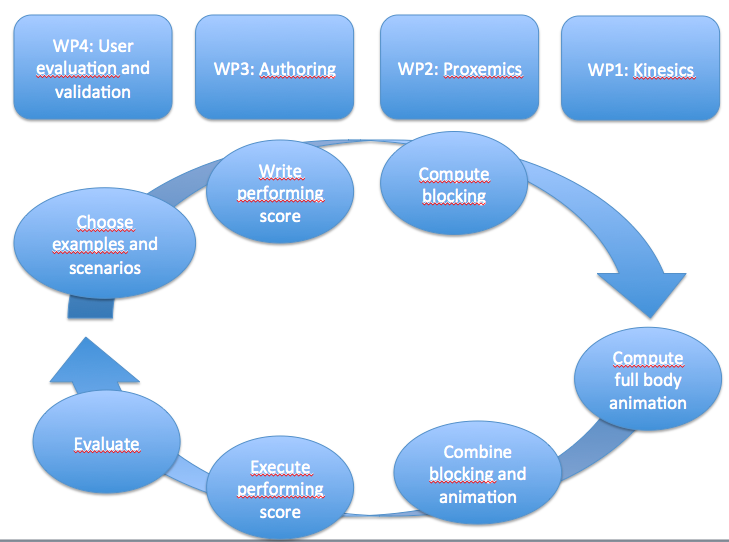
\includegraphics[width=0.8\linewidth]{DADAWORKFLOW.png}
\caption{Data flow between work packages: Through the authoring tool (WP3), a script is elaborated by a theater director (WP4); it gives direction to group of virtual
actors which act out autonomously the commands of the script to position toward each other and in the virtual space (WP2). The behaviors of each actor is computed 
taking into account their emotional states and social relations (WP1).}
\label{default}
\end{center}
\end{figure}


\endinput

% 
% \subsubsection{WP1. Related works}
% 
% Animation of an avatar is usually tackled by working separately on the full body animation model on the one hand and on the face (and gesture) animation model on the other hand (since the latter animation strongly depends on the dialogue the avatar is engaged in), where the animation produced by the two models are merged to produce a final complete animation \cite{DBLP:journals/tvcg/ShoulsonMKB14}. 
% 
% Full body kinematic animation (or control) consists in animating the full body of an avatar while he is performing actions such as walking, dancing, sitting etc. Although there has been lots of work on this subject it is still a challenging problem due to the high dimensionality of the character's configuration. Data-driven approaches are very popular here and make of use motion-capture data to learn animation models which, once learned, may be used to animate a virtual character to perform a given task. 
% Many systems have been proposed for producing animation models and controlers, they usually are based on statistical models such as Hidden Markov Models (HMMs) \cite{DBLP:journals/tog/LevineTK09} and Conditional Random Fields (CRFs) \cite{DBLP:journals/tog/LevineKTK10, DBLP:conf/atal/ChiuM14}. Most accurate methods exploit a large dataset of motions where one can synthesize a complete motion sequence corresponding to a particular task by using warping or blending strategies of motions in the training set \cite{WitkinAndPopovic1995}. Locomotion controllers have been proposed that concatenate motion
% clips from a motion capture dataset to produce an animation that is smooth [Treuille et al. 2007; Mc-Cann and Pollard 2007]. High-quality kinematic controllers have been built from this idea by using a {\it motion graph}, which is a graph structure that describe how clips from a dataset can be reordered into new motions \cite{LeeEtAl2002}. 
% While locomotion controllers are driven
% by direct high-level commands (such as desired movement direction), no such clear control signal is available for body language. To animate the face, and accompanying arm gestures, many works have focused on developing specific animation models based on a dialogue related input, either speech, text or prosody features \cite{DBLP:journals/tog/LevineTK09, DBLP:journals/tog/LevineKTK10, DBLP:conf/atal/ChiuM14, NOUS}. 
% At the end, recent work has demonstrated such models for the case of locomotion believable controllers, gesture controllers (Levine 2010) and face controllers (Ding et al., 2013). 
% % We will aim to generalize this previous work
% % to more general action controllers, including such actions as: sitting, standing, walking, grasping, taking and putting
% % objects, in a variety of expressions and moods.
% Yet all these statistical approaches require large annotated datasets to work well.
% 
% Thereby these approaches do not easily work with small training sets which is a key issue, as stressed for instance in \cite{DBLP:journals/tog/LevineWHPK12}, since first it requires considerable effort and time to build large datasets, and second because many applications demand unique motion styles and require their own datasets. This has led a number of researchers to put the effort on designing models that may be easily learned from a few samples. One main approach for doing so lies in the use (or learning) of a continuous state space to represent the data, making learning in this low dimensional space much easier  \cite{DBLP:journals/tog/LevineWHPK12, DBLP:conf/atal/ChiuM14}. A relevant technology for this are Gaussian Process which have been extended for dealing wiuth dynamic data in \cite{DBLP:journals/pami/WangFH08}.
% 
% These latter models are not far from recurent neural networks, and to Long Short Term Memory neural networks in particular \cite{DBLP:conf/nips/HochreiterS96, DBLP:journals/corr/GreffSKSS15}, that have been shown recently to work well for complex signals such as speech and handwriting, for recognition tasks \cite{DBLP:conf/nips/GravesS08} as well as for synthesis tasks \cite{DBLP:journals/corr/Graves13}. These models are part of a current trend in machine  learning called representation learning (see the recently born conference ICLR at http://www.iclr.cc/) which aims at discovering relevant and usually low dimensional representation of the data under investigation (the pionner work of this domaine is the one by G. Hinton in Science \cite{DBLP:journals/cogsci/HintonOWT06}.
% 
% 
% % High-quality kinematic con-
% % trollers have been created for tasks such as boxing [Lee and Lee
% % 2006] and locomotion [McCann and Pollard 2007; Treuille et al.
% % 2007; Lo and Zwicker 2008; Lee et al. 2009], using a discrete
% % representation of motion data called a motion graph, which uses
% % a graph structure to describe how clips from an example library can
% % be reordered into new motions [Arikan and Forsyth 2002; Kovar
% % et al. 2002; Lee et al. 2002]. 
% 
% 
% 
% % 
% % ADAPT : Interactive control of virtual characters can be
% % achieved by searching through motion clip samples for desired mo-
% % tion as an unsupervised process [Lee et al. 2002], or by extracting
% % descriptive parameters from motion data [Johansen 2009]. Proce-
% % dural methods are used to solve specific tasks such as reaching, and
% % can leverage empirical data [Liu and B 2003], example mo-
% % tions [Feng et al. 2012b], or hierarchical inverse kinematics [Baer-
% % locher and Boulic 2004] for more natural movement. Physically-
% % based approaches [Faloutsos 2002; Yin et al. 2007] derive con-
% % trollers to simulate character movement in a dynamic environment.
% % We refer to Pettr ́ et. al. [2008] for a more extensive summary of
% % work in these areas.
% 
% 
% % 
% % Real time prosody : \cite{DBLP:journals/tog/LevineTK09}
% % We present a data-driven method that automatically generates
% % body language animation from the prosody of the participant’s
% % speech signal. The system is trained on motion capture data of real
% % people in conversation, with simultaneously recorded audio. 
% % 
% % To generate the animation, we select appropriate gesture subunits
% % from the motion capture training data based on prosody cues in the
% % speech signal. 
% 
% 
% 
% % Gesture Controlers : \cite{DBLP:journals/tog/LevineKTK10}
% % Prior speech-based gesture synthesis techniques directly associate
% % animation segments with prosody features [Levine et al. 2009].
% % Such methods are sensitive to the amount and quality of training
% % data, and suffer heavily from extraneous, accidental associations,
% % known as overfitting. I
% % 
% % The development of gesture controllers was inspired by the recent
% % introduction of online locomotion controllers that assemble motion
% % clips from motion capture to produce an animation that is smooth,
% % natural, and satisfies a set of constraints [Treuille et al. 2007; Mc-
% % Cann and Pollard 2007]. While locomotion controllers are driven
% % by direct high-level commands (such as desired movement direc-
% % tion), no such clear control signal is available for body language.
% % 
% 
% % 
% % Learning few samples
% % 
% % GP pour humain motion \cite{DBLP:journals/pami/WangFH08}
% 
% % Levine :Continuous character control .. \cite{DBLP:journals/tog/LevineWHPK12} 
% % Central to a method’s ease of use is its capacity to synthesize character motion for novel
% % situations without requiring excessive data or programming effort.
% % 
% % Full body kinematic control is a challenging problem, due to the
% % high dimensionality of the character’s configuration and the diffi-
% % culty of avoiding low quality motions. High-quality kinematic con-
% % trollers have been created for tasks such as boxing [Lee and Lee
% % 2006] and locomotion [McCann and Pollard 2007; Treuille et al.
% % 2007; Lo and Zwicker 2008; Lee et al. 2009], using a discrete
% % representation of motion data called a motion graph, which uses
% % a graph structure to describe how clips from an example library can
% % be reordered into new motions [Arikan and Forsyth 2002; Kovar
% % et al. 2002; Lee et al. 2002]. However, while graphs are well suited
% % for representing large datasets, smaller datasets that lack extensive
% % transitions and variations may be inadequate to induce an expres-
% % sive discrete graph. 
% % 
% % Marsella : Gesture generation ... \cite{DBLP:conf/atal/ChiuM14}
% % 
% % 
% % Recurrent NNs:
% % Graves offline \cite{DBLP:conf/nips/GravesS08}
% % synythese handwriting \cite{DBLP:journals/corr/Graves13}
% % LSTM old \cite{DBLP:conf/nips/HochreiterS96}
% % LSTM new \cite{DBLP:journals/corr/GreffSKSS15}
% % 
% % % 
% % % Layered acting .. DOntcheva \cite{DBLP:journals/tog/DontchevaYP03}
% % 
% % 
% % Deep : 
% % Hintn 2006 \cite{DBLP:journals/cogsci/HintonOWT06}

\subsubsection{WP1. Kinesic component} 




This WP aims at creating multi-modal statistical models of an individual character's body movements from annotated data (e.g. motion capture data), to generate novel expressive animation suitable for dramatic performances. To do so we will tackle few difficult and open problems. 

First we will work at designing new full body controlers based on recent advances in statistical machine learning and on representation learning. We will focus on designing generic models allowing animation in many settings including  emotional state and actor's profile (morphology, expressivity level etc). We want in particular that, while the animation model will be learned from a limited number of actors' data, the controlers should be able to be remapped to other actors. 
Our idea is to build models that take as input few contextual variables that encode the setting (mood, actor's profile etc) as continuous input variables. 
% Designing models whose synthesized animation continuously vary with these contextual inputs naturally yield easy generalizing to unseen settings in the training set (e.g. particular combination of action, mood and actor's morphology). 
% Such generic models would allow learning the animation model for a particular action may be learned from all samples of this action whatever the mood ant the actor's morphology, and from all samples of any action performed with this particular mood.
In a first step we will extend our previous works on markovian contextual models \cite{Radenen2014, Ding2013, Ding2014} to full body animation. 
% These models are a variant of Hidden Markov Models (HMMs) that have shown strong potential for designing speech-based face controllers, where speech features are the contexual variables that infuence the way the face is animated. 
Next, we will investigate the use of continuous state space models and particularly of (deep) recurrent neural networks. Such models, and some of their variants, have been proposed recently for diffcult recognition tasks on complex signals (e.g. speech \cite{DBLP:journals/taslp/Abdel-HamidMJDPY14}) as well as on synthesis tasks for handwriting \cite{DBLP:journals/corr/Graves13}. These frameworks are part of the representation learning line of work which brought impressive breakthrough in few machine learning tasks for signals, speech recognition \cite{DBLP:conf/interspeech/Abdel-HamidDYJ13,DBLP:journals/spm/LingKZSSQMD15} as well as in computer vision tasks \cite{DBLP:journals/nn/Schmidhuber15, DBLP:conf/eccv/LeCun12}. 
% The main difficulty lies here in imagining ways to integrate the idea of using contextual variales in these models in order to integrate contextual information that would modify the behaviour of the models. 
Finally we plan to explore fully new alternative strategies such as using neuro muscular based models following ideas of deltalognormal models from \cite{DBLP:conf/icfhr/FischerPOS14}. Such a modeling allows recovering the sequence of neuromuscular commands that generated a handwritten gesture. Although these models led to impressive results in terms of modeling accuracy, these models have been applied to very simple gestures only and their ability to handle complex gestures is not certain. Yet if we were able to make them robust enough to provide valuable interprettation of complex motion, these models would bring in our opinion a very promising line of research for building new and natural motion controllers. 

% Next we will have to combine multiple animation models in order to take advantage of all existing works, in particular for the animation of the face. 
% Controlling a fully-articulated character is traditionally accomplished using a series of interwoven subcomponents responsible for various parts of the body. We will mainly distinguish between the body animation and the face animation.




% Thierry : parler plutot de 3 verrous scientifiques. We will organize the work in three tasks, the two first tasks are dedicated to modeling and synthesizing animations. We will distinguish between animating the whole body and animating the face which will be animated based on a given scenario but also based on the scenario from other actors to enable accurate interaction between actors (e.g. gazes). Why ? The last task is focused on making the models designed in thee two first tasks able to learn from few training data

% A first scientific lock lies in the design of generic body controllers able to synthesize the animation of the full body of a character for many settings (combination of action, emotion and actor's profile). 
% It is an elegant way for producing smooth animation of complex motions which usually requires artifical smoothing and postprocessing. It is also a relevant modeling framework for learning from limited datasets. 
% Indeed gathering a dataset including enough training samples for every combination of (action, emotion, actor profile) is unlikely. 
% Defining generic models should allow to maximize the exploitation of the training data for learning, which is a key issue here. 


% % The idea is to build models that take as input contextual variables that encode the setting in such a way that the animation model for a particular action may be learned from all samples of this action whatever the mood, and from all samples of any action performed with this particular mood.
% One main idea for doing so consists in extending to full body animation the idea of contextual models \cite{Radenen2014, Ding2013, Ding2014} which are a variant of Hidden Markov Models (HMMs) that have shown strong potential for designing face controllers. 
% Contextual HMMs are HMMs whose parameters (means of Gaussian distribution transition probabilities etc), are defined as a (learned) function of contextual variables. One Contextual HMM may be viewed as a continuum of HMMs, one model for every possible value of contextual variables.
% These models will serve as a baseline. Next, we will investigate the use of continuous state space models and particularly of (deep) recurrent neural networks. Such models have shown strong abilities for dealing with complex signals like speech and handwriting \cite{DBLP:journals/corr/Graves13}. 
% The main difficulty lies here in imagining ways to integrate the idea of using contextual variales in these models in order to integrate contextual information that would modify the behaviour of the models. 
% Finally we plan to explore alternative strategies such as using neuro muscular based models following ideas like the one of deltalognormal models from \cite{DBLP:conf/icfhr/FischerPOS14} which allow recovering the sequence of neuromuscular commands that generated a handwritten gesture. 

% We will also investigate new ways for parameterizing the animation model with few variables related to the emotional state of an actor and more generally to an actor’s profile. The difficulty here lies in the definition of defining the representation of an actor, we will attempt to learn it directly from data using recent techniques named as representation learning (Contardo 2014). 

A second lock will concern the animation of the face in dialogue situations. Given that we have worked previously with three complementary methods, we will focus here on how to mix our face animation models: a mocap based animation model \cite{DBLP:conf/icassp/DingRAP13,Ding2014}, a video-based animation model \cite{Barbulescu2014}, and the procedural animation model in the GRETA system  \cite{greta}. The main issue here will be to imagine efficient frameworks for inferring based on the scenario of the animation which model to use or combine to produce a final animation.

% The mocap based animation model will be easily built on previous works by the team \cite{YuThesis}. 
% Finally starting from previous work on visual prosody we will design the third model ... Ideally, this should be done without MOCAP data, using only audio and video processing, possibly enhanced with depth (kinect). To be continued (Rémi)...We will explore strategies for optimally combining these three animation models...


Finally we want our animation models to be easily extendable to new activities, gestures and moods, by making them learnable from only few training samples. This  will allow enriching the system easily whitout a costly and tedious task of gathering a large corpus of training data as usually required in statistical machine learning. Learning statistical models from few samples is an open issue, it has ony been adressed in few studies for simple gestures like handwriting signals \cite{ArtieresPAMI07} \cite{NIPS2013_OneShot}.  We will go beyond these preliminary studies and will explore few ways that aim at favoring transfer from learning one action / mood model to learning another action / mood model. 
In particular we will explore strategies for modifying our generic controlers, e.g. based on recurrent neural networks or on contextual markovian models \cite{Radenen2014}, in order to enable transfer learning between action models so that a new action model can be learned with only few samples of this action. 
% Second we will mix the idea of continuous state space models and of dimension reduction to design low dimensional state space Reccurrent neural nets. Projecting the dynamics of an action move in such a low dimensional space should permit characterizing it much easier, enabling learning from few samples. 


% We will mainly investigate two approches for extending approaches developped in task T11 to enable learning from few samples. The first strategy consists in extending the idea of context variables that models of task T11 rely on in order to design a global model for all actions.
% In the case of markovian model for instance this means that instead of definig one model per action one could define a unique big markovian model where every state would stand for a particular position of the body and performing an action would correspond to following a path (i.e. a state sequence) in this big model. The model for a particular action would correspond then in a bundle of paths in this model.  Doing so one could expect that all the training data (whatever the action it corresponds to) could be exploited to learn all the states of this big markovian model, hence implementing some kind of transfer learning between actions. A new action would correspond then in a bundle of paths in this model and could be learnt from few samples only. Preliminary works that we did let us expect that such a strategy would work with statistical markovian models (Ding et al., 2013). In this case the above idea is implementing by introducing new contextual variables, which are indicators of the action to perform, 
% that modify the gaussian densities. We will first investigate this strategy deeper for contextual markovien models then we will extend this approach to neural networks. 
% 
% Second we will explore the use of using continuous state space models with a low dimensional state space (e.g. corresponding to the degree of freedom of body poses or to the neuro muscular commands) which should permit characterizing a particular motion or gesture as its dynamic in this latent space whose limited dimension would enable learning from few samples.  




\endinput


\subsubsection{WP2. Proxemic component: procedural animation models for interaction between actors.}

Previous works on modeling group formation have been mainly applied to ECAs and have focused on the spatial positioning and orientation of the ECAs \cite{Pedica2010}. Few researches have looked at modeling group of ECAs with different personalities and social attitudes \cite{Gillies2004,Prada2005}. However these models do not consider the dynamic evolution of the group behaviors nor how do the actors' behaviours synchronize with each other. In this task, we focus on simulating group of autonomous actors interacting with each other where each actor is defined by its emotional state and its relation toward others and objects. Social relations can be represented by two dimensions, affiliation and dominance \cite{Wiggins1979}. We will extend group behavior model \cite{Pedica2010} that embeds the F-Formation proposed by Kendon \cite{Kendon2004} to consider social relations and emotional states of actors. 

Physical distance between actors, their body orientation toward each other, gaze direction, facial expression, gesture expressivity are cues of the relation with others and with objects and of emotional states. These cues will be embedded in the proxemics component. They evolve continuously in relation to the others' behaviors. To simulate the dynamic evolution of these behaviors we will make use of Neural Network simulation \cite{Prepin2013} where we can render how behaviors of one actor can act on behaviors of other actors (eg walking powerfully toward an actor with an angry expression will result in moving backward of another actor with a less dominant attitude. Mutual coupling of behaviors will be modeled as emerging from such action-reactive behavior simulation \cite{Prepin2013} ensuring not only the synchronization between actors' behaviors but also their mutual influence. This task will be led by Telecom ParisTech with the contribution of Inria.



\endinput

\subsubsection{WP3. Performance authoring and real-time execution. }

This work package will elaborate a common conceptual framework for assembling all the behaviors, goals and animations of all actors into a coordinated, real time performance. Based on this framework, we will develop software tools for authoring the performance and controlling it in real-time. Authoring of performances will be based on traditional cue sheet, which are familiar to theatre directors (Gagner\'e 2012, Ronfard 2012). Cue-sheet are multi-modal documents consisting of blocking notations  written in a pseudo-natural language of verbs and adverbs, together with a graphical annotation providing spatial and temporal cue signals  for all actor movements, using stage views and floor plan views. A cue-sheet provides a convenient notation of stage directions, which can be easily created and edited by directors, and used a specification for a virtual performance. Internally, we will compile the cue sheet into a hierarchical finite-state machine, which is a de-facto standard in real-time game engines. 

We will take advantage of the motion models created in WP1 and WP2 to create finite-state machines with a rich vo-cabulary of high-level actor behaviors, suitable for generating complex performances. Following (Mateas 2002), we will decompose the input cue-sheet into minimal units of behaviors (beats ) organized as one state-machine per actor, all connected together, and one state-machine for a stage manager  controlling the advancement of the storyline. Depending on their current states, virtual actors will update their positions, orientations and gaze directions using be-haviors from WP2, and their other animation parameters using procedural models from WP1. 

All software tools developed in WP1 and WP2 will thus be integrated into a common runtime, playable in the Unity game engine, and used in WP4 for evaluation and validation. This task will be led by Inria, with contributions from all partners.

\endinput



\subsubsection{WP4. Evaluation and validation.  }

This task will insure the integration of the research prototype within the cultural context of creative industries and artis-tic practices. Using the autonomous digital actors from WP1, WP2 and WP3, Paris 8 will create short theatre scenes covering the spectrum of actions and emotions covered by the project. The directorial constraints will be adapted to the research scope in order to guarantee expressive results matching creative issues. A survey of teachers and creators from theater, dance, cinema, digital art, video game of Paris 8 creative environment will help to design the prototype in the direction of users' needs. Evaluation and validation will include short staged performances targeting different application areas, including theatre, pantomime, staging of chorists in opera, as well as previsualization of movie scenes and simulation of non player characters in video games. It will aim at a high expressive level of realization and give feed-back on the quality of animation and the usability of the 
authoring tools offered for directing virtual actors in those contexts. This task will be supervised by Paris 8 with contributions from members of the Labex Arts-H2H leading project Process of directing actors  which involves international stage directors teachers and students of the Conservatoire National Sup\'erieur d'Art Dramatique (CNSAD ' National theater school).

\endinput


\subsection{Management du projet / Project management}
\begin{xcomment}  
Pr\'eciser les aspects organisationnels du projet et les modalit\'es de coordination (si possible individualisation d'une tâche de coordination).
\end{xcomment}


The project will be coordinated by Inria with a collegial decision-making process. A steering committee composed of Thierry Arti\`eres (LIF), 
Georges Gagner\'e (Paris 8), Catherine Pelachaud (LITC) and R\'emi Ronfard (Inria) will make all important decisions  in unanimity. 
The committee will meet before every consortium meeting and its decisions will be 
communicated to all consortium members and to ANR. R\'emi Ronfard will be the project coordinator and will be responsible for applying
the decisions of the steering committee and for communicating with ANR and other consortium members. 

%In cases  of disagreements,  a compromise will have to be found. 

Consortium meetings will be organized four times a year for a total of 14 meetings, including kick-off meeting and final review meeting. 
Meetings will take place in the theatre department at Paris 8 to ensure continuity and visibility of the project in the theatre arts world. Paris is also 
a convenient meeting place for all project members. Ensuring regular meetings with all researchers involved in the project is an important
factor for success, given the widely multidisciplinary aspect of the project. This will also favour joint work by the PhD students working
on the project, and ensure their commitment to the user evaluation phase that will take place in Paris 8 as well. 

Software development will be coordinated by Inria and Paris 8 using rapid prototyping methods (SCRUM) \footnote{SCRUM is a popular
and established technique in the game industry, which is applicable to DADA. SCRUM facilitates agile software development
with a small team of part-time developers and a dynamic team organization}. The project coordinator, R\'emi Ronfard,
will act as the "Scrum Master", taking responsibility for the delivery of software increments during fast-paced development periods (including, but not limited to 
the project milestones). C\'edric Plessiet will act as the "Product Owner", taking responsibility for the specifications and selection of features included in each increment,
for the deployment of all software increments at Paris 8, for their testing and user evaluations, and for filling bug reports and user documentations.

All PHD Students will be asked to contribute their latest results to be included in the DADA prototype at least twice a year. 
The rest of their time will be devoted to their research work. Source code files will be signed by all contributing authors, 
together with their affiliations, to properly  track intellectual property rights.



\endinput



\subsection{Description des travaux par tâche / Description by task}
\begin{xcomment}  
Pour chaque tâche, d\'ecrire : 
les objectifs et \'eventuels indicateurs de succ\`es,
les personnes impliqu\'ees,
le programme d\'etaill\'e des travaux,
les livrables,
les contributions des personnes (le qui fait quoi ),
la description des m\'ethodes et des choix techniques et de la mani\`ere dont les solutions seront apport\'ees,
les risques et les solutions de repli envisag\'ees.
\end{xcomment}


\subsubsection{WP1 Kinesics}

\paragraph{Task11}  Choosing representations for full body motion ; representation learning ; transfer learning ; parameterisation of kinesic components. This can include neuro-muscular variables ; also the choice of kinematic trees rooted at the head ; also the grouping of kinematic variables into synergies ; etc. 

One classical distinction is between world-frame positions and joint angle variables In our case, we are making a strong statement that we will  study kinesic variables for all joints relative to the rigid body frame associated with the actor. This could be the ground floor position of the actor plus a rigid body position associated with the actor?s head.  Thus proxemic variables could be footsteps and head movements ; kinesic variables could be all other joint angles or joint positions in world coordinates.

\paragraph{Task12} Learning bi-dimensional models of actions and moods from a mocap dataset of six actions (walk, carry object, knock on door, throw object, lift object, move object) in 8 moods (neutral, happy, afraid, angry, anxious, sad, proud, shameful). Ideally, we would like to separate the action components from the mood components of motion and extrapolate the moods to other actions, and the actions to other moods. 

\paragraph{Task13} Learning models of gesture and facial expressions in dialogue situations.
Based on previous work on  visual prosody, we would like to learn joint models of gesture and  speech prosody. Ideally, this should be done without MOCAP data, using only audio and video processing, possibly enhanced with depth (kinect).

\paragraph{Task14}  Learning parameterized kinesic models. 

Bbecause our models are contextual, conditioned by the proxemic components, we should be able to change their velocity,  amplitude, direction and phase (in the way of parametric HMM models). This is challenging and needs to be investigated. 


\subsubsection{WP2 Proxemics}

\paragraph{Task 21} Group behaviors during multi-way conversation ; turn-taking ; synchronization of actors in dialogue ; implementation of conversational phenomena (interruption, pause, re-run, repetition, etc.)

\paragraph{Task 22} Group behaviors during stage movements ? implementation of advanced steering behaviors  such as follow, flee, separate, join, merge, enter stage, exit stage, etc. 

Create better models by taking gaze and head movement into account ; Physical models of social interactions ; implementation of action-reaction chains between actors ; 

\paragraph{Task 23} High level models of actions and reactions, timing, implementation of theatrical effects. Provoke surprise and/or expectation, etc. Models of tri-partite interaction between two actors and the audience in dialogue and in movement. Theatrical cheating techniques. '

\paragraph{Task 24}  Combination of statistical and procedural models ; smooth transitions between action keeping the same mood; between moods keeping the same action ; smooth transitions between dialogue and action ; adaptation to proxemic contexts.


\subsubsection{WP3 Authoring}

\paragraph{Task31} Specification of a dramatic language of verbs (actions, speech acts, movements) and adverbs (moods, attitudes, dramatic effects) for directing actors ; define cues as synchronisation points between actors ; define parallel and sequential behaviors ; etc.

Part of this language will be devoted to stage blocking / movement

Part of this language wil be devoted to dialogue

\paragraph{Task32}  Compilation of the language into a finite state machine and/or Petri net ; allowing real-time execution of the dramatic score ; user interface for directing actors by sketching stage floor plans and composing the dramatic score ; one line per actor per motion component (proxemic behaviors, kinesic actions, kinesic moods, speech acts, etc.)

\paragraph{Task33} Real-time execution of the dramatic score ; real-time combination of proxemic (procedural) and kinesic components of motion ; non-deterministic motion generation ; synchronization to cues ; real-time skinning and advanced 3D animation ; integration of physically-based secondary animation (skin, hair, clothes, etc.)

This includes integration of the GRETA BML realizer with IMAGINE animation ; and real-time integration of the statistical models of motion with the procedural animation components.


\paragraph{Task 34} User adaptation.
Allow director to add corrections and let system learn the differences using imitation learning or active learning or other related techniques ; etc.


\subsubsection{WP4 User evaluation and validation}

\paragraph{Task41} Scenarios.

Writing scenes with didascalia 
Dialogue scenes with groups of 2, 3 and 4 actors using a choice of didascalia
Silent stage movements, as in opera synched to music, using a choice of didascalia
Alternations of dialogue and stage movements in theatre scenes with 2 actors

\paragraph{Task42} Validation of the interaction.

Is the dramatic language adequate ? useful ?  efficient  ? 

Is the dramatic score interface  adequate ? useful ?  efficient  ? 

Is the stage floor plan sketching tool adequate ? useful ?  efficient  ? 

\paragraph{Task43} Validation of the animation

Dialogue scenes  with groups of 2, 3 and 4 actors.

Silent stage movements of groups of 2, 3 and 4 actors, as in opera synched to music

Combination of dialogue and action for scenes with 2 actors



Notes


If needed, we could try to learn models of gesture and proxemics from video by learning gesture controllers \cite{Levine2010},
using  our previous work in actor and action recognition, including

Daniel Weinland, Remi Ronfard, Edmond Boyer. Automatic Discovery of Action Taxonomies from Multiple Views. IEEE Conference on Computer Vision and Pattern Recognition (CVPR) - 2006. 

D Weinland, E Boyer, R Ronfard. Action recognition from arbitrary views using 3d exemplars. International Conference on Computer Vision, 2007. ICCV 2007.

V Gandhi, R Ronfard.   Detecting and naming actors in movies using generative appearance models. Computer Vision and Pattern Recognition (CVPR), 2013.


Learning head-driven kinesic animation could be done following the line of 

Sreenivasa, Soueres, Laumond, Berthoz ; Steering a humanoid robot by its head. Intelligent Robots and Systems, 2009.

Combining proxemics and kinesics components could be done along the lines of

Hironori Mitake, Kazuyuki Asano, Takafumi Aoki, Marc Salvati, Makoto Sato, Shoichi Hasegawa : 'Physics-driven Multi Dimensional Keyframe Animation for Artist-directable Interactive Character', Computer Graphics Forum, Vol.28, No.2, pp.279-287, 2009.





\subsection{Calendrier des tâches, livrables et jalons / Tasks schedule, deliverables and milestones}
\begin{xcomment} 
Pr\'esenter sous forme graphique un \'ech\'eancier des diff\'erentes tâches et leurs d\'ependances (diagramme de Gantt par exemple).
Pr\'esenter un tableau synth\'etique de l'ensemble des livrables du projet (num\'ero de tâche, date, intitul\'e, responsable).
Pr\'eciser de façon synth\'etique les jalons scientifiques et/ou techniques, les principaux points de rendez-vous, les points bloquants ou al\'eas qui risquent de remettre en cause l'aboutissement du projet ainsi que les r\'eunions de projet pr\'evues.

\end{xcomment}

\endinput



\section{Strat\'egie de valorisation, de protection et d'exploitation des r\'esultats / Dissemination and exploitation of results. intellectual property}
\begin{xcomment}   
A titre indicatif : 2 pages maximum pour ce chapitre.
Pr\'esenter les strat\'egies de valorisation des r\'esultats :
la communication scientifique,
la communication aupr\`es d'autres communaut\'es scientifiques et du grand public, notamment la promotion faite à la culture scientifique et technique. Si un budget sp\'ecifique est pr\'evu à cet effet, le sp\'ecifier et l'identifier dans une tâche de la proposition (voir § 3.1).
les r\'esultats attendus en mati\`ere de valorisation,
les retomb\'ees scientifiques, techniques, industrielles, \'economiques, '
la place du projet dans la strat\'egie industrielle des entreprises partenaires du projet,
les autres retomb\'ees (normalisation, information des pouvoirs publics, formation dans l'enseignement sup\'erieur, ...),
les \'ech\'eances et la nature des retomb\'ees technico-\'economiques attendues,
l'incidence \'eventuelle sur l'emploi, la cr\'eation d'activit\'es nouvelles, '

Pr\'esenter les grandes lignes des modes de protection et d'exploitation des r\'esultats.
\end{xcomment}


\endinput



\section{Description de l'equipe / Team description}
\begin{xcomment}  
A titre indicatif : 2 pages maximum pour ce chapitre.
\end{xcomment}

% 


\subsection{Description, ad\'equation et compl\'ementarit\'e des participants / Partners description, relevance and complementarity}
\begin{xcomment}  
Fournir les \'el\'ements permettant d'appr\'ecier la qualification des personnes impliqu\'ees dans la proposition de projet (le pourquoi qui fait quoi ). Il peut s'agir de r\'ealisations pass\'ees, d'indicateurs (publications, brevets), de l'int\'erêt pour le projet'
Montrer la compl\'ementarit\'e et la valeur ajout\'ee des coop\'erations entre les diff\'erents participants. 
Le cas \'ech\'eant, l'interdisciplinarit\'e et l'ouverture à diverses collaborations seront à justifier en accord avec les orientations du projet.
\end{xcomment}

The consortium involves three research teams with complementary experience in computer graphics, intelligent virtual agents and statistical machine learning and a research team in theatre studies. Telecom ParisTech and University of Marseille are already working together on facial animation from speech through the co-supervision of Yu Ding's thesis (Ding 2013). Inria/Imagine and Paris 8 are also already working together on directing audiovisual prosody of actors, as part of Ad\'ela Barbulescu thesis (Barbulescu 2014). Results of the two theses will be exploited in the project.






\subsection{Qualification du coordinateur du projet / Qualification of the project coordinator}
\begin{xcomment} 
0,5 page maximum
Fournir les \'el\'ements permettant de juger la capacit\'e du coordinateur à coordonner le projet.
\end{xcomment}


Remi Ronfard is a computer scientist with a 20 year experience in industry and academia in France, Canada and USA. He has worked at the T.J. Watson IBM Research Center in New York as post-doc and as a visiting scientist (1992 and 2000).  He is now a member of the IMAGINE research team at Inria and the University of Grenoble, where his research is devoted to designing novel interfaces between artists and  computers. He is the author of 4 international patents and more than 60 scientific papers published in top ranked international journals (IJCV, CVIU, PAMI) and conferences (Siggraph, Eurographics, CVPR, ICCV, ECCV)  and cited more than 4000 times.  He will be acting as coordinator for DADA.

Remi was trained as an engineer then PhD student at Mines Paris Tech. He  has conducted research in a variety of domains, including digital storyboarding (INA, 1995), aesthetic surface design (IBM Research and Dassault Syst�mes, 2000), video indexing (INA, 2000), action recognition and statistical analysis of image and film styles (INRIA 2002-2007). He was an expert in the international MPEG group from 1997 to 2000. In 2007, he became a team leader at Xtranormal Technologies. His  team created the patented ?magicam? system, which was used to produce two million user-generated 3D animation movies. He came back to INRIA in 2009 with a new research program devoted to  ?directing virtual worlds?. He helped to create the IMAGINE team in 2012,  where he now  leads the ?narrative design? part of the project. Towards this goal, he investigates computational models of visual storytelling. This has led to inspiring collaborations with the national  film school (ENS Louis Lumi�re) and the C�lestins Theatre in Lyon. He 
has  co-chaired international workshops on modeling people and human interaction (Beijing, 2005), 3-D cinematography (New York City, 2006; Banff, 2008; Providence, 2012), intelligent cinematography and editing (Quebec, 2014). He is currently serving as head of the ?Geometry and Image? Department at Laboratoire Jean Kuntzmann, Univ.  Grenoble Alpes.



\subsection{Qualification, rôle et implication des participants / Qualification and contribution of each partner}
\begin{xcomment}  
(1 page maximum)
Qualifier les personnes, pr\'eciser leurs activit\'es principales  et leurs comp\'etences propres.

Pour chacune des personnes dont l'implication dans le projet est sup\'erieure à 25\% de son temps sur la totalit\'e du projet (c'est-à-dire une moyenne de 3 hommes.mois par ann\'ee de projet), une biographie d'une page maximum sera plac\'ee en annexe du pr\'esent document qui comportera :
Nom, pr\'enom, âge, cursus, situation actuelle
Autres exp\'eriences professionnelles
Liste des cinq publications (ou brevets) les plus significatives des cinq derni\`eres ann\'ees, nombre de publications dans les revues internationales ou actes de congr\`es à comit\'e de lecture.
Prix, distinctions
Si besoin, pour chacune des personnes, leur implication dans d'autres projets (Contrats publics et priv\'es effectu\'es ou en cours sur les trois derni\`eres ann\'ees) sera pr\'esent\'ee et fournie en annexe du pr\'esent document. On pr\'ecisera l'implication dans des projets europ\'eens ou dans d'autres types de projets nationaux ou internationaux. Expliciter l'articulation entre les travaux propos\'es et les travaux ant\'erieurs ou d\'ejà en cours.

\end{xcomment}
\begin{table}
\begin{tabularx}{ \textwidth}{| p{2cm} | p{2cm} |p{2cm} |  p{2cm} |  p{2cm} |  p{1cm} |  X |    }
\hline
Partner &Name & First name & Position & Field of research & PM & Contribution  \\
\hline
LIF & Arti\`eres& Thierry & Pr & Machine Learning & 14 & WP1 (task leader), WP2, WP3 \\
\hline
LIF & Emyia & Valentin & Assistant Pr& Machine Learning and Signal Processing & 5 & WP1 \\
\hline
LIF & Qi& Wang& Ph.D. student & Machine Learning  & 12 & WP1 \\
\hline

\end{tabularx}

\caption{Qualification and contribution of each partner}
\end{table}

\paragraph{INRIA EPI IMAGINE}

IMAGINE stand for: "Intuitive Modeling and Animation for Interactive Graphics \& Narrative Environments". The challenge we aim to address is the efficient, interactive creation of animated 3D content. To this end, our goal is to develop a new generation of knowledge-based models for shapes, motions and stories. These models will embed both procedural methods, enabling the fast generation of high quality content, and intuitive control handles, enabling users to easily convey their intent and to progressively refine their result. These models will be used within different interactive environments dedicated to specific applications. More precisely, we will apply our work to three main domains: shape modeling, motion synthesis and narrative design. In addition to addressing specific needs of digital artists, this research should in the long term, enable professionals and scientists to represent and interact with models of their objects of study, and educators to quickly express and convey their ideas.  
Our international scientific partners include UC Berkeley, UBC, the University of  Toronto, McGill and ETHZ and Disney Research Zurich. 

In adddition to Remi Ronfard, two other permanent  researchers and a post-doctoral student will actively participate to the DADA project.

{\bf Marie-Paule Cani} is a full-time professor at INPG and director of the IMAGINE team. She will contribute to DADA 
with her recent work on implicit skinning, advanced hair style rendering, advanced clothe adaptation, etc. 

{\bf Damien Rohmer} is an associate member of the IMAGINE team. He will contribute to DADA with his recent work on
implicit skinning ? physically-based animation ? 

{\bf Adela Barbulescu} is a third-year Phd student who will work part-time on the DADA project during her post-doc in 2016.
She will contribute to DADA with her recent work on visual prosody, which will be extended for joint generation of speech
and facial animation from directorial input. 


\paragraph{ECM} Two main researchers from the QARMA team will participate to the project. 

{\bf Thierry Arti\`eres} is a professor at University of Aix-Marseille, and a member of the {\it QARMA team} (eQuipe AppRentissage et Multimédia) at LIF (Laboratoire d’Informatique Fondamentale). One of his major research topic concerns machine learning for multimedia applications, more particularly for sequences and signals, either for classification, pattern discovery, sequence labeling and sequence synthesis, with strong experience with various signals such as speech, bioacoustics, handwriting, gestures, eye movements, WII signals, Kinect and motion capture data. He is author or co-author of about sixty papers and articles in top ranked international conferences (NIPS, ICML, AISTAT, ICASSP, EMNLP) and journals (IEEE PAMI, JMLR, Pattern Recognition) in the fields of theoretical as well as applied machine learning (speech and handwriting recognition, user modeling) and artificial intelligence.  

{\bf Valetin Emiya} is assistant professor in the QARMA team at LIF since 2011. He has conducted research in audio processing and sparse models for 8 years and has strong connexion with the signal processing group at I2M Lab in Marseille. His current works on models and algorithms for audio inpainting (see \cite{Adler2012, Adler2011} and project ANR JCJC MAD), i.e. interpolation and extrapolation in audio sequences. This works are currently being extended to the extrapolation of gesture for the control of electronic musical instrument and contemporary music creation, through the Progest project by GdR ISIS (2014-2016) in collaboration with the gmem Centre National de Cr\'eation Musicale (\url{http://www.gmem.org/index.php?option=com_content&view=article&id=5580144&Itemid=13660}).
 
 
{\bf Wang Qi} is a first-year Phd student whose research topic on recurrent neural networks for signal processing tasks is related to the project. He will contribute to DADA mainly on WP1 (tasks 1.1 and 1.3). 

\paragraph{Paris 8}

{\bf Georges Gagner�} is a lecturer in performing arts at the University Paris 8 where he teaches acting in digital environments. As part of Labex Arts H2H, he is an active member of two projects�on  ��Actor directing as art creation process�� (La direction d?acteurs comme processus de cr�ation artistique), and ��Augmented scenery�� (La Sc�ne Augment�e). He is also a stage director and member of the collaborative platform didascalie.net, focusing on real time intermedia environments in performing arts.  In 2007, he initiated the research project ANR VIRAGE about methods and software prototypes for cultural industries and for the arts. He is involved in the OSSIA and INEDIT ANR project through the realization of the artistic project ParOral, based on digital shadows direction through the voice, with the Iscore software. He directed productions in national theaters (Th��tre National de Strasbourg, La Filature, Sc�ne nationale de Mulhouse, Th��tre G�rard Philipe, Centre dramatique national de Saint-Denis) and organized numerous workshops on the impact of real time new technologies on theater and scenic writings. He collaborates with St�phane Braunschweig and Peter Stein as stage director first assistant on more than 20 differents opera productions in the most famous european theaters (La Scala, La Fenice, Th��tre des Champs-Elys�es, L'Op�ra Comique, Le Festival International d'Art Lyrique d'Aix-en-Provence, La Monnaie de Bruxelles, L'Op�ra de Lyon, L'Op�ra du Rhin, etc.). 

{\bf C�dric Plessiet} is an associate professor at University Paris 8  where he teaches special fx game programming, Unity 3D programming and computer art. Before that, he has worked with special effects and motion capture companies, creatin virtual semi-autonomous butterfly actor for prize-winning movie "four wings and a pryer". His research interests include movie and theatre previz, real-time game engine programming and artificial intelligence for video games. His computer  art projects have been featured at the Futur En Seine, Paris FX and IVRC conferences. He  has worked with the international Buto dancer Atsuchi Takenuchi. His art was presented in London, Rumania Switzerland and Japan (http://www.mobilisimmobilis.com/, http://ivrc.net/2006/, http://www.symposium-pi.ch/)

{\bf Jean-Fran�ois Dusigne} is  professor of Paris 8 University, and ex-actor of Th��tre du Soleil (Ariane Mnouchkine). He will bring his international expertise on the different ways of directing actors, and the transmission issues.

{\bf Isabelle Moindrot} is the  director of the ARTS H2H Labex. She  will help to the integration of DADA in the global artistical research ecosystem of Paris 8.

{\bf Martial Poirson} is a professor at Paris 8 University, and director of the theatre departement. He will help to the dissemination of the DADA's deliverables though the academic and professional fields.


\paragraph{LTCI} LTCI (Laboratoire de Traitement et Communication de l?Information) is a joint laboratory between CNRS and TELECOM ParisTech (UMR 5141). It hosts all the research efforts of TELECOM ParisTech (a faculty of about 150 full-time staff (full professors, associate and assistant professors), 30 full time researchers from CNRS and 300 Ph.D students). Its disciplines include all the sciences and techniques that fall within the term "Information and Communications": Computer Science Networks, Communications, Electronics, Signal and Image Processing, as well as the study of economic and social aspects associated with modern technology. 

{\bf Catherine Pelachaud} is Director of Research at CNRS in the laboratory LTCI, TELECOM ParisTech. She received her PhD in Computer Graphics at the University of Pennsylvania, Philadelphia, USA in 1991. Her research interest includes representation languages for agents, embodied conversational agents, nonverbal communication (face, gaze, and gesture), expressive behaviours and multimodal interfaces. She has been involved and is still involved in several European projects related to multimodal communication (EAGLES, IST-ISLE), to believable embodied conversational agents (IST-MagiCster, FP5 PF-STAR), emotion (FP5 NoE HUMAINE, FP6 IP CALLAS, FP7 STREP SEMAINE) and social behaviours (FP7 NoE SSPNet, H2020 Aria-Valuspa).

{\bf Chlo� Clavel} is Assistant Professor at Telecom Paristech. She owned a PhD on acoustic analysis of emotional speech. Before joining Telecom ParisTech she worked as a researcher at Thales Research and Technology where she focused on emotion analysis; then she became a researcher at EDF R \& D working on sentiment analysis and opinion mining. She has participated to several collaborative projects and has coordinated one national project.

{\bf Yu Ding} is a post-doctoral student at LTCI. He has obtained his PhD in September 2014 under the supervision of Thierry Arti�res and Catherine Pelachaud. His topics of interest are to develop data-driven approach for expressive animation of virtual agents.


\endinput



\section{Justification scientifique des moyens demand\'es / Scientific justification of requested ressources}
\begin{xcomment}  
On pr\'esentera ici la justification scientifique et technique des moyens demand\'es dans le document de soumission tel que synth\'etis\'e et rempli en ligne sur le site de soumission dans la fiche tableaux r\'ecapitulatifs  du document administratif et financier tel que rempli en ligne sur le site de soumission.
Justifier les moyens demand\'es en distinguant les diff\'erents postes de d\'epenses.
(2 pages maximum)
\end{xcomment}


Budget: We request a financial aid of 518  K\euro for three PhD students  and two post-doctoral students,  computer hardware and software, and
travel expenses (50 K\euro). The project duration should be 42 months in order to develop a functional prototype in three years 
and to use it to animate several play scripts for evaluation and validation purposes.









\subsection{\'Equipement / Equipment}
\begin{xcomment}  
Pr\'eciser la nature des \'equipements* et justifier le choix des \'equipements (un devis pourra être demand\'e si le projet est retenu pour financement).
Dans le cas où les achats doivent être compl\'et\'es par d'autres sources de financement, indiquer le montant et l'origine de ces aides compl\'ementaires, et le pourcentage demand\'e à l'ANR sur le pr\'esent projet.
\end{xcomment}


LTCI request 12 500 \euro{}  to  cover equipments (High performance PC with good graphics card), publication fees for open-access journals, 
some software and research books.

The theater laboratory EA1573 asks for 4000 \euro{} for the purchase of a working station and all the softwares and hardwares necessary for the development of the WP4.

\subsection{Personnel / Staff}
\begin{xcomment}  
Le personnel non permanent (th\`eses, post- doctorants, CDD...) financ\'e sur le projet devra être justifi\'e.
Fournir  les profils des postes à pourvoir pour les personnels à recruter.

Pour les th\`eses, pr\'eciser si des demandes de bourse de th\`ese sont pr\'evues ou en cours, en pr\'eciser la nature et la part de financement imputable au projet. 
\end{xcomment}

LTCI requets a financial aid of 108 K\euro{}  for a PhD. 


The theater research team EA1573 asks for two Post-Doc of 12 months each (40k \euro{} per Post-Doc). In collaboration with the INREV team, the first post-doc 
will intervene on the WP4.2 to guarantee an effective communication between the WP3 and the WP4  but also to help in the software implementation of experiments, documentation by tutorial, sample and user's manual. The second post-doc will intervene on the WP4.3 to bring to a successful conclusion of the dramatic  score, to build complex animation, and to help in the validation of the prototype whether it is from a qualitative and quantitative point of view with the spectators, the actors and the users of the software. It will also have for mission to finalize the user set of documents to guarantee the distribution of the system to other potential users (video games, performing arts, etc.)

%\subsection{Prestation de service externe / Subcontracting}
%\begin{xcomment}  
%Pr\'eciser:
%la nature des prestations,
%le type de prestataire.
%\end{xcomment}

\subsection{Missions / Travel}
\begin{xcomment} 
Pr\'eciser :
les missions li\'ees aux travaux d'acquisition sur le terrain (campagnes de mesures'),
les missions relevant de colloques, congr\`es'
\end{xcomment}

To participate to project meetings, exchange visit of PhD student and participation to national and international conferences, a budget of 15K \euro{}  per partner  is needed
for LTCI, Inria and LIF. Paris 8 requests  4000 \euro{}  in spawn of mission to allow the researchers mobilized to exchange with the partner labs, but also to present their research in various colloquiums and festivals (Ars Electronica, Laval Virtual, Les bains num�riques, SIGGRAPH Art Sessions). Theater laboratory asks for 4000 \euro{}
to finance external expertises of the theater field to help in the validation of the deliverables.

%\subsection{D\'epenses justifi\'ees sur une proc\'edure de facturation interne / Costs justified by internal procedures of invoicing}
%\begin{xcomment}  
%Pr\'eciser la nature des prestations.
%\end{xcomment}
%Not applicable.
%
%\subsection{Autres d\'epenses de fonctionnement / Other expenses}
%\begin{xcomment}
%Toute d\'epense significative relevant de ce poste devra être justifi\'ee.
%\end{xcomment}
%Not applicable.




\endinput



%\newpage
\section{Bibliographie / References}
\small 
%\footnotesize
\sanstitre
\bibliography{dada_science}

\end{document}
 
